\documentclass[11pt, a4paper]{article}

\usepackage{style}

\institution{EPFL}
\project{Project CSE I}
\title{Notes}
\author{Fabio Matti}
\supervisor{Prof. Fabio Nobile \\ Dr. Davide Pradovera}
\date{\today}

\begin{document}

\maketitle

\section{Finite element method}
\label{sec:fem}

\subsection{The general approach}
\label{subsec:theory}

\textit{Summarizes Chapter 1 in Quarteroni: Introduction to Finite Elements Method}

Usually, the problems may be expressed in a simple equation 

\begin{equation}
    \begin{cases}
        L u = f & in~\Omega \\
        u = u_D & on~\partial \Omega
    \end{cases}
    \label{equ:strong}
\end{equation}

where $L$ denotes a linear differential operator (e.g. $-\Delta$ in the Poisson
equation), $u$ the solution to be found, and $f$ is a source term independent
of $u$. Some boundary condition $u_D$ is imposed on the solution $u$.

However, equation (\ref{equ:strong}) usually does not allow all physically
significant solutions (particularly non-differentiable ones). Therefore, we convert 
the problem to a weak form. This is achieved by multiplying (\ref{equ:strong}) with 
a test function $v \in V$, and integrating over the whole domain $\Omega$:

\begin{equation}
    \int_{\Omega} (L u) v = \int_{\Omega} f v, ~\forall v \in V \label{equ:initialweak}
\end{equation}

Usually, integration by parts allows us to \enquote{transfer} the derivatives from 
the $L u$ term to the test function $v$, such that the order (with respect to 
the derivatives taken) is more \enquote{balanced} between the two terms. As a
trade-off, a boundary term appears and needs to be eliminated to facilitate the 
finite element solution. This term can often be eliminated by restricting ourselves
to test functions from a subspace $V' \subset V$. The weak problem then reads

\begin{equation}
    \int_{\Omega} (L_u u) (L_v v) = \int_{\Omega} f v, ~\forall v \in V' \label{equ:weak}
\end{equation}

with a linear differential operator $L_u$ acts on the solution $u$, and a linear 
differential operator $L_v$, appearing due to the integration by parts, acts on 
the test function $v$. For simplicity, we refer to the left-hand side as the 
bilinear form

\begin{equation}
    a(u, v) = \int_{\Omega} (L_u u) (L_v v)
\end{equation}

and the right-hand side as the linear form

\begin{equation}
    F(v) = \int_{\Omega} f v
\end{equation}

To solve (\ref{equ:weak}), we prefer to look for approximate solutions $u_h$ in a finite 
dimensional space $V_h$ with $dim(V_h) = N_h$ \textcolor{red}{(what role does $V_h'$,
the space wherein $v$ lies to satisfy the boundary conditions, play? as far as I can tell
$V_h'$ is the subspace of $V_h$, in which all functions vanish at the boundary where
$u$ is known)}. Choosing a basis $\{\varphi_i\}_{i \leq N_h}$
then allows us to represent the approximate solution as 

\begin{equation}
    u_h = \sum_{j \leq N_h} u_j \varphi_j
\end{equation}

for some coefficients $u_i$ that need to be determined. We thus see, that 
(\ref{equ:weak}) turns into a linear system, since we only need to test the 
equality for the basis elements $\varphi_i$ of $V_h$:

\begin{equation}
    \sum_{j=1}^{N_h} u_j a(\varphi_j, \varphi_i) = F(\varphi_i),~i \in \{1, \dots, N_h\}
\end{equation}

If we write $A_{ij} = a(\varphi_j, \varphi_i)$ and $\mathbf{F} = (F(\varphi_1), \dots, F(\varphi_{N_h}))^T$,
we have reduced the problem to finding $\mathbf{u} = (u_1, \dots, u_{N_h})^T$,
such that 

\begin{equation}
    \mathbb{A}\mathbf{u} = \mathbf{F}
\end{equation}

and have identified an approximate solution to (\ref{equ:strong}) as
$u \approx u_h = \sum_{j \leq N_h} u_j \varphi_j$.

Choosing the space $V_h$ is fundamental to have an accurate method that 
gives a good approximation $u_h$ of $u$. Furthermore, the choice of basis 
$\{\varphi_i\}_{i \leq N_h}$ influences how $\mathbb{A}$ ends up looking.
Of particular interest are bases for which $a(\varphi_j, \varphi_i)$ vanishes 
for almost all $i$ and $j$, thus yielding a sparse matrix $\mathbb{A}$. The
choice of basis also controls the conditioning of $\mathbb{A}$
\textcolor{red}{(need to find an example to illustrate this)}.

\subsection{The Poisson equation}
\label{subsec:poisson}

\textit{Taken from FEniCS manual (too lazy for bibtex...)}

We aim to solve an equation of the form

\begin{equation}
    - \Delta u(\mathbf{x}) = f(\mathbf{x}) \label{equ:poisson}
\end{equation}

on a domain $\mathbf{x} \in \Omega$, with a solution $u(\mathbf{x})$
that satisfies a certain boundary condition $u(\mathbf{x}) = u_d(\mathbf{x})$
for all $x \in \partial \Omega$ that lie on the border of $\Omega$.

To do this, we first convert this equation to its weak form
by multiplying both sides with a arbitrary test function
$v(\mathbf{x})$, which vanishes on the border (i.e. $v(mathbf{x}) = 0, \forall
\mathbf{x} \in \partial \Omega$), and by then integrating over all of $\Omega$:

\begin{equation}
    - \int_{\Omega} \Delta u(\mathbf{x}) v(\mathbf{x}) d\mathbf{x} = \int_{\Omega} f(\mathbf{x}) v(\mathbf{x}) d\mathbf{x} 
\end{equation}

We may now rearrange the gradient product rule $\nabla (a b) = (\nabla a) b + a (\nabla b)$ and
Gauss' theorem (as long as $v(x)$ is differentiable in a neighborhood of $\Omega$)
combined with the fact that $v(\mathbf{x})$ vanishes on $\partial
\Omega$ to convert the right-hand side to

\begin{align}
    - \int_{\Omega} \Delta u(\mathbf{x}) v(\mathbf{x}) d\mathbf{x} &= - \int_{\Omega} \nabla ( \nabla u(\mathbf{x}) v(\mathbf{x}) ) d\mathbf{x} + \int_{\Omega} \nabla u(\mathbf{x}) \nabla v(\mathbf{x}) d\mathbf{x} \notag \\ 
    &= - \int_{\partial \Omega} \nabla u(\mathbf{x}) v(\mathbf{x}) d\boldsymbol{\omega} + \int_{\Omega} \nabla u(\mathbf{x}) \nabla v(\mathbf{x}) d\mathbf{x} \notag \\ 
    &= \int_{\Omega} \nabla u(\mathbf{x}) \nabla v(\mathbf{x}) d\mathbf{x}
\end{align}

Consequently, the weak formulation of the problem is to find $u(\mathbf{x})$, such
that for arbitrary $v(\mathbf{x})$, we have

\begin{equation}
    \int_{\Omega} \nabla u(\mathbf{x}) \nabla v(\mathbf{x}) d\mathbf{x} = \int_{\Omega} f(\mathbf{x}) v(\mathbf{x}) d\mathbf{x}
\end{equation}

To simplify and generalize the notation, we may use the linear form $L:V \to \mathbb{R}$ as 

\begin{equation}
    L(v) = \int_{\Omega} f(\mathbf{x}) v(\mathbf{x}) d\mathbf{x}
\end{equation}

and also the bilinear form $a: V \times V \to \mathbb{R}$

\begin{equation}
    a(u, v) = \int_{\Omega} \nabla u(\mathbf{x}) \nabla v(\mathbf{x}) d\mathbf{x}
\end{equation}

\subsection{Example: One dimensional Poisson equation}
\label{subsec:1dpoiss}

\textit{Initial idea taken from Wikipedia article about FEM.}

To illustrate the choice of basis functions, we will now consider the simple one 
dimensional case $\Omega = [a, b]$, such that the weak formulation of the problem
turns into 

\begin{equation}
    \int_a^b u'(x) v'(x) dx = \int_a^b f(x) v(x) dx
\end{equation}

We now subdivide the domain $[a, b]$ into $M$ subintervals, each of length
$h=(b - a)/M$, with nodes at $x_k = a + hk, k \in \{0, 1, \dots, M\}$. We
proceed to choose as the basis functions the class of the piecewise linear
Lagrange interpolating polynomials on $[x_k, x_{k+1}], k \in \{0, 1, \dots, M\}$,
defined as 

\begin{equation}
    v_k(x) = \frac{x-x_{k-1}}{x_{k}-x_{k-1}} \mathbf{1}_{\{x \in [x_{k-1}, x_k]\}} + 
            \frac{x_{k+1}-x}{x_{k+1}-x_k} \mathbf{1}_{\{x \in [x_k, x_{k+1}]\}}
\end{equation}

If we now interpolate $f(x)$ and $u(x)$ as piecewise linear Lagrange polynomaials,
we get the representation

\begin{align}
    f(x) &\approx \sum_{i=1}^{M} f(x_{i-1})\frac{x-x_{i}}{x_{i-1} - x_{i}} + f(x_i)\frac{x-x_{i-1}}{x_{i} - x_{i-1}} \notag \\
     &= \sum_{i=1}^{M-1} f(x_i)v_i(x)
\end{align}

and analogously

\begin{equation}
    u(x) = \sum_{i=1}^{M-1} u(x_i)v_i(x)
\end{equation}

We now restricted ourselves to the discrete variational formulation of the problem

\begin{equation}
    \sum_{i=1}^{M-1} u(x_i) \int_a^b v_i'(x) v_j'(x) dx = \sum_{i=1}^{M-1} f(x_i) \int_a^b v_i(x) v_j(x) dx
\end{equation}

which needs to be satisfied for all $j \in \{0, 1, \dots, M\}$.

This equation can be rewritten in terms of two matrices $\mathbf{K}$ and $\mathbf{L}$
which we define as

\begin{align}
    K_{ij} &= \int_a^b v_i(x) v_j(x) dx \\
    L_{ij} &= \int_a^b v_i'(x) v_j'(x) dx
\end{align}

such that we get

\begin{equation}
    \sum_{i=1}^{M-1} u(x_i) L_{ij} = \sum_{i=1}^{M-1} f(x_i) K_{ij}
\end{equation}

Notice, that we only need the entries $K_{ij}$ and $L_{ij}$ with
$i \in \{1, 2, \dots, M-1\}$, since we already know the boundary conditions 
of $u(x)$ at $x = x_0$ and $x = x_M$.

We realize, that the $L_2$ inner product of $v_i(x)$ with $v_j(x)$ (and
consequently also the one of $v_i'(x)$ with $v_j'(x)$) is zero for
all $|i-j| > 1$, hence, we distinguish two different cases.

\begin{enumerate}
    \item $i = j$: Here, the inner product turns out to be
    \begin{align}
        \int_a^b v_i(x) v_i(x) dx &= \int_{a}^{b} \left(\frac{x-x_{i-1}}{x_{i}-x_{i-1}} \right)^2 \mathbf{1}_{\{x \in [x_{i-1}, x_i]\}} + 
        \left(\frac{x_{i+1}-x}{x_{i+1}-x_i}\right)^2 \mathbf{1}_{\{x \in [x_i, x_{i+1}]\}} dx \notag \\ 
        &= 2 \int_{x_{i-1}}^{x_i} \left(\frac{x-x_{i-1}}{x_{i}-x_{i-1}} \right)^2 dx \notag \\ 
        &= \frac{2}{h^2} \int_{x_{i-1}-x_{i-1}}^{x_i - x_{i-1}} u^2 du \notag \\
        &= \frac{2}{h^2} \frac{1}{3} h^3 \notag \\
        &= \frac{2h}{3} \notag \\
     \end{align}
     and for the derivatives it is
     \begin{align}
        \int_a^b v_i'(x) v_i'(x) dx &= \int_{a}^{b} \left(\frac{1}{x_{i}-x_{i-1}} \right)^2 \mathbf{1}_{\{x \in [x_{i-1}, x_i]\}} + 
        \left(\frac{-1}{x_{i+1}-x_i}\right)^2 \mathbf{1}_{\{x \in [x_i, x_{i+1}]\}} dx \notag \\ 
        &= 2 \int_{x_{i-1}}^{x_i} \left(\frac{1}{x_{i}-x_{i-1}} \right)^2 dx \notag \\ 
        &= \frac{2}{h^2} \int_0^h 1 du \notag \\
        &= \frac{2}{h}
     \end{align}
    \item $|i - j| = 1$: Here, we can limit ourselves to the case where $j = i+1$,
    since the other case is fully symmetric. We calculate
    \begin{align}
        \int_a^b v_i(x) v_{i+1}(x) dx &= \int_{a}^{b} \frac{x_{i+1}-x}{x_{i+1}-x_i} \frac{x-x_i}{x_{i+1}-x_i} \mathbf{1}_{\{x \in [x_i, x_{i+1}]\}} dx \notag \\ 
            &= \int_{x_i}^{x_{i+1}} \frac{x_{i+1}-x}{x_{i+1}-x_i} \frac{x-x_i}{x_{i+1}-x_i} dx \notag \\ 
            &= \frac{1}{h^2} \int_{x_i-x_i}^{x_{i+1}-x_i} (x_{i+1}-x_i-u) u du \notag \\ 
            &= \frac{1}{h^2} \int_0^h (h - u) u du \notag \\
            &= \frac{1}{h^2} (\frac{h^3}{2} - \frac{h^3}{3}) \notag \\ 
            &= \frac{h}{6}
    \end{align}
    and for the derivative it is 
    \begin{align}
        \int_a^b v_i'(x) v_{i+1}'(x) dx &= \int_{a}^{b} \frac{-1}{x_{i+1}-x_i} \frac{1}{x_{i+1}-x_i} \mathbf{1}_{\{x \in [x_i, x_{i+1}]\}} dx \notag \\ 
            &= -\frac{1}{h^2} \int_{x_i}^{x_{i+1}} 1 dx \notag \\ 
            &= -\frac{1}{h}
    \end{align}
\end{enumerate}

Now, using the previously defined matrices $\mathbf{K}_{ij}$ and 
$\mathbf{L}_{ij}$, we get the matrix equation 

\begin{equation}
    \mathbf{L}u = \mathbf{K}f
\end{equation}

with 

\begin{align}
    u &= (u_0, u(x_1), \dots, u_M)^T \\
    f &= (f(x_0), f(x_1), \dots, f(x_{M}))^T \\
    \mathbf{L} &= \begin{pmatrix}
        1 & & & & \\
        \frac{2}{h} & -\frac{1}{h} & & & \\
        -\frac{1}{h} & \frac{2}{h} & -\frac{1}{h} & & \\
        & -\frac{1}{h} & \frac{2}{h} & \ddots & & \\
        & & -\frac{1}{h} & \ddots  & -\frac{1}{h} \\
        & & & \ddots & \frac{2}{h} \\
        & & & & 1 \\
    \end{pmatrix} \\
    \mathbf{K} &= \begin{pmatrix}
        \frac{u_0}{f(x_0)} & & & & \\
        \frac{2h}{3} & \frac{h}{6} & & & \\
        \frac{h}{6} & \frac{2h}{3} & \frac{h}{6} & & \\
        & \frac{h}{6} & \frac{2h}{3} & \ddots & & \\
        & & \frac{h}{6} & \ddots  & \frac{h}{6} \\
        & & & \ddots & \frac{2h}{3} \\
        & & & & \frac{u_M}{f(x_M)} \\
    \end{pmatrix} \\
\end{align}

Here, we have adjusted the first rows in $\mathbf{L}$ and $\mathbf{K}$, such that
the boundary conditions are necessarily satisfied.
To obtain the finite element solution, we simply solve this linear system.

\section{Maxwell's equations}
\label{sec:maxwell}

Let $\mathbf{E} = (E_1, E_2, E_3)^T$ denote the electric field,
$\mathbf{B} = (B_1, B_2, B_3)^T$ the magnetic field strength, and 
$\mathbf{j} = (j_1, j_2, j_3)^T$ the electric current density. 
We suppose Maxwell's equations hold:

\begin{align}
    \nabla \cdot (\epsilon \mathbf{E}) &= \rho \label{equ:mw1} \\
    \nabla \cdot \mathbf{B} &= 0 \label{equ:mw2} \\
    \nabla \times \mathbf{E} &= -\partial_t \mathbf{B} \label{equ:mw3} \\
    \nabla \times (\mu^{-1} \mathbf{B}) &= \partial_t (\epsilon \mathbf{E}) + \mathbf{j} \label{equ:mw4}
\end{align}

\subsection{Vector potential formulation}
\label{subsec:vectorpot}

We can therefore use (\ref{equ:mw2}) to write $\mathbf{B} = \nabla \times \mathbf{A}$ for some vector
potential $\mathbf{A}$. Furthermore, we can identify from (\ref{equ:mw3}) that
$\mathbf{E} = -\nabla \phi - \partial_t \mathbf{A}$ can be written for some
scalar potential $\phi$.

The physical quantities $\mathbf{E}$ and $\mathbf{B}$ remain unchanged 
if we transform $\mathbf{A} \to \mathbf{A}' = \mathbf{A} + \nabla \psi$ and
$\phi \to \phi' = \phi - \partial_t \psi$ (gauge transformations), 
as can be explicitly verified by plugging these transformed potentials into the
definitions of $\mathbf{E}$ and $\mathbf{B}$. Choosing as the gauge field as 

\begin{equation}
    \psi = \int_0^t \phi dt'
\end{equation}

we see that $\phi' = \phi - \partial_t \int_0^t \phi dt' = \phi - \phi = 0$.
Hence, if we now express the electric field $\mathbf{E}$ in terms of these transformed 
potentials, we realize that $\mathbf{E} = -\nabla \phi' - \partial_t \mathbf{A}' = -\partial_t \mathbf{A}'$
because we have transformed $\phi$ exactly in such a way, which makes $\phi'$ vanish
(not symbolically, but due to its actual value being zero).
As for the magnetic field $\mathbf{B}$, we have $\mathbf{B} = \nabla \times \mathbf{A}'$.

Plugging these identities into (\ref{equ:mw4}), and for simplicity replacing 
the symbol $\mathbf{A}'$ with $\mathbf{A}$ again, we get
 
\begin{equation}
    \nabla \times (\mu^{-1} \nabla \times \mathbf{A}) = - \epsilon
    \partial_t^2 \mathbf{A} + \mathbf{j} \label{equ:mwvecpot}
\end{equation}

We may want to introduce a harmonic time dependence
of $\mathbf{A}$ and $\mathbf{j}$ with frequencies $\omega$, such that $\mathbf{A}(\mathbf{x}, t) = 
\mathbf{A}(\mathbf{x})\exp(i \omega t)$ and $\mathbf{j}(\mathbf{x}, t) = 
\mathbf{j}(\mathbf{x})\exp(i \omega t)$. Plugging this into (\ref{equ:mwvecpot})
yields us

\begin{equation}
    \nabla \times (\mu^{-1} \nabla \times \mathbf{A}) -  \epsilon \omega^2 \mathbf{A} = \mathbf{j} \label{equ:mwtimeharm}
\end{equation}

We reduce this equation to its weak formulation, by multiplying it with a vector-valued 
function $\mathbf{v} \in H_{\text{curl}}(\Omega)$, where we denoted

\begin{equation}
    H_{\text{curl}}(\Omega) = \{u : \Omega \to \mathbb{C}, ~\text{such that}~ u \in L^2(\mathbb{C})^3,
    \nabla \times u \in L^2(\mathbb{C})^3 \}
\end{equation}

and by integrating over all of $\Omega$:

\begin{equation}
    \int_{\Omega} (\nabla \times ({\mu^{-1} \nabla \times \mathbf{A}})) \cdot \mathbf{v}
    - \epsilon \omega^2 \int_{\Omega} \mathbf{A} \cdot \mathbf{v} = \int_{\Omega} \mathbf{j} \cdot \mathbf{v} \label{equ:mwweak}
\end{equation}

To further simplify this expression, we will derive an identity for the scalar product
of a vector-valued function $\mathbf{v}$ with the curl of a vector-valued function 
$\mathbf{u}$. For this, we use the completely antisymmetric tensor $\varepsilon_{ijk}$
(frequently referred to as the Levi-Civita tensor), to rewrite the $k$-th component
of the curl as

\begin{equation}
    (\nabla \times \mathbf{u})_k = \sum_i \sum_j \varepsilon_{ijk} \partial_i u_j
\end{equation}

where $\partial_i$ denotes the partial derivative with respect to the $i$-th coordinate
direction. Rewriting the scalar product as a sum and identifying $\mathbf{u} = \mu^{-1}
\nabla \times \mathbf{A}$, we apply the product rule to get

\begin{align}
    (\nabla \times \mathbf{u}) \cdot \mathbf{v} &= \sum_k (\nabla \times \mathbf{u})_k v_k \notag \\ 
    &= \sum_k (\sum_i \sum_j \varepsilon_{ijk} \partial_i u_j) v_k \notag \\ 
    &= \sum_k \sum_i \sum_j \partial_i (\varepsilon_{ijk} u_j v_k) - \sum_k \sum_i \sum_j u_j (\varepsilon_{ijk} \partial_i v_k) \notag \\ 
    &= \sum_k \sum_i \sum_j \partial_i (\varepsilon_{jki} u_j v_k) - \sum_k \sum_i \sum_j u_j ((-\varepsilon_{ikj}) \partial_i v_k) \notag \\ 
    &= \sum_i \partial_i (\mathbf{u} \times \mathbf{v})_i + \sum_j u_j (\nabla \times \mathbf{v})_j \notag \\ 
    &= \nabla \cdot (\mathbf{u} \times \mathbf{v}) + \mathbf{u} \cdot (\nabla \times \mathbf{v}) \label{equ:curlidentity} 
\end{align}

Consequently, we may rewrite the double curl term as 

\begin{align}
    \int_{\Omega} (\nabla \times ({\mu^{-1} \nabla \times \mathbf{A}})) \cdot \mathbf{v} &=
    \int_{\Omega} \nabla \cdot (({\mu^{-1} \nabla \times \mathbf{A}}) \times \mathbf{v})
    + \int_{\Omega} ({\mu^{-1} \nabla \times \mathbf{A}}) \cdot (\nabla \times \mathbf{v}) \notag \\
    &= \int_{\partial \Omega} (({\mu^{-1} \nabla \times \mathbf{A}}) \times \mathbf{v}) \cdot \mathbf{n}
    + \int_{\Omega} ({\mu^{-1} \nabla \times \mathbf{A}}) \cdot (\nabla \times \mathbf{v}) \notag \\
\end{align}

Again denoting $\mathbf{u} = \mu^{-1} \nabla \times \mathbf{A}$, we can rearrange 

\begin{align}
    (\mathbf{u} \times \mathbf{v}) \cdot \mathbf{n} &= \sum_k (\sum_i \sum_j \varepsilon_{ijk} u_i v_j) n_k \notag \\
     &= \sum_j (\sum_i \sum_k (-\varepsilon_{ikj}) u_i n_k) v_j \notag \\ 
     &= - (\mathbf{u} \times \mathbf{n}) \cdot \mathbf{v} 
\end{align}

and therefore have

\begin{equation}
    \int_{\partial \Omega} (({\mu^{-1} \nabla \times \mathbf{A}}) \times \mathbf{v}) \cdot \mathbf{n}
    = - \int_{\partial \Omega} (({\mu^{-1} \nabla \times \mathbf{A}}) \times \mathbf{n}) \cdot \mathbf{v}
\end{equation}

We can finally identify the weak form of the problem as

\begin{equation}
    \int_{\Omega} ({\mu^{-1} \nabla \times \mathbf{A}}) \cdot (\nabla \times \mathbf{v})
    - \epsilon \omega^2 \int_{\Omega} \mathbf{A} \cdot \mathbf{v} 
    = \int_{\Omega} \mathbf{j} \cdot \mathbf{v}
    + \underbrace{\int_{\partial \Omega} (({\mu^{-1} \nabla \times \mathbf{A}}) \times \mathbf{n}) \cdot \mathbf{v}}_{\text{boundary integral term}} \label{equ:mwweaksimple}
\end{equation}

where $\mathbf{n}$ denotes the normal vector to $\partial \Omega$. Notice how we placed
the boundary integral term on the right hand side, since along the border 
$\partial \Omega$ we usually either know $\nabla \times \mathbf{A} = \mathbf{B} = \mathbf{B}_D$
(or even only $\mathbf{B} \times \mathbf{n}$) as the Neumann boundary condition
or $-i \omega \mathbf{A} = \mathbf{E}_D$ as the Dirichlet boundary condition.

\subsection{Electric field formulation}
\label{subsec:electricfield}

Multiplying both sides of (\ref{equ:mw3}) with $\mu^{-1}$ and taking the curl
allows us to substitute (\ref{equ:mw4}) in, such that we get 

\begin{align}
    \nabla \times (\mu^{-1} \nabla \times \mathbf{E})
    &= - \partial_t (\nabla \times (\mu^{-1} \mathbf{B})) \notag \\
    &= - \partial_t (\partial_t (\epsilon \mathbf{E}) + \mathbf{j}) \notag \\
    &= - \partial_t^2 (\epsilon \mathbf{E}) + \partial_t \mathbf{j}
\end{align}

Introducing a harmonic time dependence
of $\mathbf{E}$ and $\mathbf{j}$ with frequencies $\omega$, such that $\mathbf{E}(\mathbf{x}, t) = 
\mathbf{E}(\mathbf{x})\exp(i \omega t)$ and $\mathbf{j}(\mathbf{x}, t) = 
\mathbf{j}(\mathbf{x})\exp(i \omega t)$, we obtain 

\begin{align}
    \nabla \times (\mu^{-1} \nabla \times \mathbf{E}) - \omega^2 \epsilon \mathbf{E} = i \omega \mathbf{j}
\end{align}

The $i$ on the right-hand side is giving me (and most likely FEniCS too) a major
headache, hence why I will try my luck with finding a formulation involving 
$\mathbf{B}$ in the next section.

\subsection{Magnetic field formulation}
\label{subsec:magneticfield}

Multiply both sides of (\ref{equ:mw4}) with $\epsilon^{-1}$ and take the curl to obtain,
with the help of (\ref{equ:mw3}), the expression

\begin{align}
    \nabla \times (\epsilon^{-1} \nabla \times (\mu^{-1} \mathbf{B}))
    &= \nabla \times (\partial_t \mathbf{E} + \epsilon^{-1} \mathbf{j}) \notag \\ 
    &= \partial_t (\nabla \times \mathbf{E}) + \nabla \times (\epsilon^{-1} \mathbf{j}) \notag \\ 
    &= -\partial_t^2 \mathbf{B} + \nabla \times (\epsilon^{-1} \mathbf{j})
\end{align}

Introducing a harmonic time dependence
of $\mathbf{B}$ and $\mathbf{j}$ with frequencies $\omega$, such that $\mathbf{B}(\mathbf{x}, t) = 
\mathbf{B}(\mathbf{x})\exp(i \omega t)$ and $\mathbf{j}(\mathbf{x}, t) = 
\mathbf{j}(\mathbf{x})\exp(i \omega t)$, we obtain 

\begin{equation}
    \nabla \times (\epsilon^{-1} \nabla \times (\mu^{-1} \mathbf{B})) - \omega^2 \mathbf{B}
    = \nabla \times (\epsilon^{-1} \mathbf{j})
\end{equation}

Converting this equation to its weak form by multiplying both sides with a
vector valued function $\mathbf{v} \in H_{\text{curl}}(\Omega)$ and integrating
over all of $\Omega$ yields

\begin{equation}
    \int_{\Omega} (\nabla \times (\epsilon^{-1} \nabla \times (\mu^{-1} \mathbf{B}))) \cdot \mathbf{v}
    - \omega^2 \int_{\Omega} \mathbf{B} \cdot \mathbf{v}
    = \int_{\Omega} (\nabla \times (\epsilon^{-1} \mathbf{j})) \cdot \mathbf{v}
\end{equation}

Using the above derived identity

\begin{equation}
    (\nabla \times \mathbf{u}) \cdot \mathbf{v}
    = \nabla \cdot (\mathbf{u} \times \mathbf{v})
    + \mathbf{u} \cdot (\nabla \times \mathbf{v})
\end{equation}

we may write using Gauss' theorem

\begin{align}
    \int_{\Omega} (\nabla \times (\epsilon^{-1} \nabla \times (\mu^{-1} \mathbf{B}))) \cdot \mathbf{v}
    &= \int_{\Omega} \nabla \cdot ((\epsilon^{-1} \nabla \times (\mu^{-1} \mathbf{B})) \times \mathbf{v}) \notag \\ 
    &+ \int_{\Omega} (\epsilon^{-1} \nabla \times (\mu^{-1} \mathbf{B})) \cdot (\nabla \times \mathbf{v}) \notag \\ 
    &= \int_{\partial \Omega} ((\epsilon^{-1} \nabla \times (\mu^{-1} \mathbf{B})) \times \mathbf{v}) \cdot \mathbf{n} \notag \\ 
    &+ \int_{\Omega} (\epsilon^{-1} \nabla \times (\mu^{-1} \mathbf{B})) \cdot (\nabla \times \mathbf{v}) \notag \\ 
\end{align}

and 

\begin{align}
    \int_{\Omega} (\nabla \times (\epsilon^{-1} \mathbf{j})) \cdot \mathbf{v}
    &= \int_{\Omega} \nabla \cdot ((\epsilon^{-1} \mathbf{j}) \times \mathbf{v})
    + \int_{\Omega} (\epsilon^{-1} \mathbf{j}) \cdot (\nabla \times \mathbf{v}) \notag \\ 
    &= \int_{\partial \Omega} ((\epsilon^{-1} \mathbf{j}) \times \mathbf{v}) \cdot \mathbf{n}
    + \int_{\Omega} (\epsilon^{-1} \mathbf{j}) \cdot (\nabla \times \mathbf{v})
\end{align}

Since $(\mathbf{u} \times \mathbf{v}) \cdot \mathbf{n} = \mathbf{u} \cdot (\mathbf{v} \times \mathbf{n})$
(as was shown above), the boundary integrals vanish if we have

\begin{equation}
    \mathbf{v} \times \mathbf{n} = 0, ~\text{on}~\partial\Omega
\end{equation}

In that case, we end up with the following (simplified) weak form

\begin{equation}
    \int_{\Omega} (\epsilon^{-1} \nabla \times (\mu^{-1} \mathbf{B})) \cdot (\nabla \times \mathbf{v})
    - \omega^2 \int_{\Omega} \mathbf{B} \cdot \mathbf{v}
    = \int_{\Omega} (\epsilon^{-1} \mathbf{j}) \cdot (\nabla \times \mathbf{v})
\end{equation}

\section{Waveguides}
\label{sec:waveguides}

In Section \ref{sec:maxwell} we have derived the weak form of the time-harmonic
Maxwell equation for the vector potential $\mathbf{A}$. Let us now apply it to
a small collection of illustrative examples.

\subsection{Two-dimensional open-ended waveguide}
\label{subsec:2dwaveguide}

Consider a two-dimensional rectangular box of length $l$ and width $w$ enclosing
a vacuum (depicted in Figure \ref{fig:waveguide}).

\begin{figure}[h]
    \centering
    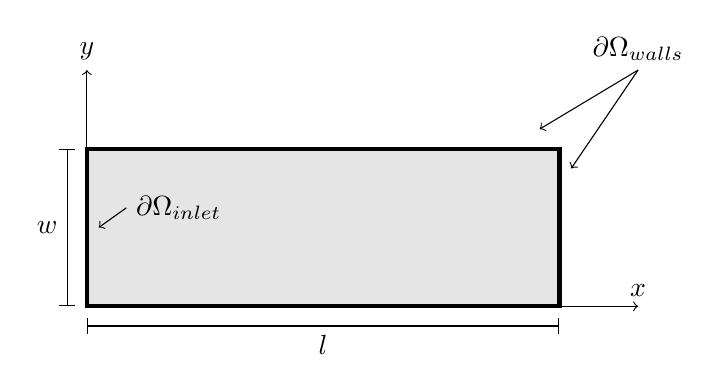
\begin{tikzpicture}
        \draw[->] (0, 0) to (0, 3) node[above] {$y$};
        \draw[->] (0, 0) to (7, 0) node[above] {$x$};
        \draw[|-|] (0, -0.25) to node[below] {$l$} (6, -0.25);
        \draw[|-|] (-0.25, 0) to node[left] {$w$} (-0.25, 2);
        \fill[black!10!white] (0, 0) rectangle (6, 2);
        \draw[ultra thick] (6, 2) rectangle (0, 0);
        \draw[<-] (6.15, 1.75) to (7, 3);
        \draw[<-] (5.75, 2.25) to (7, 3) node[above] {$\partial \Omega_{\text{walls}}$};
        \draw[<-] (0.15, 1) to (0.5, 1.25) node[right] {$\partial \Omega_{\text{inlet}}$};
    \end{tikzpicture}
    \caption{Waveguide}
    \label{fig:waveguide}
\end{figure}

Defining $\mathbf{g} = ({\mu^{-1} \nabla \times \mathbf{A}}) \times \mathbf{n} =
\mu^{-1} \mathbf{B} \times \mathbf{n}$ on the boundary $\partial \Omega$
and setting $\mathbf{j} = 0$, we can convert (\ref{equ:mwweaksimple}) into

\begin{equation}
    \int_{\Omega} (\mu^{-1} \nabla \times \mathbf{A}) \cdot (\nabla \times \mathbf{v})
    - \epsilon \omega^2 \int_{\Omega} \mathbf{A} \cdot \mathbf{v} 
    = \int_{\partial \Omega} \mathbf{g} \cdot \mathbf{v} \label{equ:mwweakwaveguide}
\end{equation}

If we only consider $\mathbf{A} = (0, 0, A_z)^T$ and $\mathbf{v} = (0, 0, v_z)^T$,
the two curls can be rewritten as the dot product of two gradients, since 

\begin{equation}
    \nabla \times \mathbf{A} = (\partial_y A_z, -\partial_x A_z, 0)
\end{equation}

and similarly for $\nabla \times \mathbf{v}$, such that

\begin{equation}
    (\nabla \times \mathbf{A}) \cdot (\nabla \times \mathbf{v}) = (\nabla A_z) \cdot (\nabla v_z)
\end{equation}

We thus end up with the following simplified weak form of the problem

\begin{equation}
    \int_{\Omega} (\mu^{-1} \nabla A_z) \cdot (\nabla v_z)
    - \epsilon \omega^2 \int_{\Omega} A_z v_z
    = \int_{\partial \Omega} g_z v_z \label{equ:mwweakwaveguidesimple}
\end{equation}

\subsubsection{Constant field (old and flawed version)}
\label{subsubsec:constfieldold}

Suppose we observe an electromagnetic wave at frequency $\omega$ and with the magnetic 
field of strength $B_0$ aligned with the $y$-direction incident on the waveguide
at $x=0$. Symbolically, we thus have $\mathbf{B}(t) = (0, B_0, 0)^T \exp(i \omega t)$
at $x=0$ for $y \in [0, w]$.

From this, we can calculate the function $g_z$ on the \enquote{inlet} boundary to be 
(knowing that we have already taken account of the harmonic time-dependence of 
$\mathbf{B}$ in deriving (\ref{equ:mwweakwaveguidesimple}))

\begin{equation}
    \mathbf{g}_{\text{inlet}} = \mu^{-1} \mathbf{B} \times \mathbf{n} = \mu^{-1} B_0 (\mathbf{e}_y \times \mathbf{e}_x) = -\mu^{-1} B_0 \mathbf{e}_z
\end{equation}

Referring to Section \ref{subsec:boundary}, we know that for perfectly conducting 
walls the magnetic field $\mathbf{B}$ in our case (with walls on top and bottom)
must satisfy 

\begin{equation}
    n \cdot \mathbf{B} = 0 ~ \implies ~ B_y = 0
\end{equation}

This, in turn, means that \textcolor{red}{different orientation of $\mathbf{n}$
for bottom wall!}

\begin{equation}
    \mathbf{g}_{\text{walls}} = \mu^{-1} \mathbf{B} \times \mathbf{n} = \mu^{-1} B_x (\mathbf{e}_x \times e_y) = \mu^{-1} B_x e_z
\end{equation}

Therefore, in general, we have (assuming all other walls to be perfect conductors) 

\begin{equation}
    g_z = \begin{cases} -\mu^{-1} B_0, & \text{at the inlet} \\ 0 & \text{at the walls} \end{cases}
\end{equation}

\textcolor{red}{Ok, this is not entirely right, because this implicitly assumes that 
$B_x = 0$ at the walls (which would be correct for purely transversal waves in the
waveguide, but not in general). Will somehow have to find a way to  correct this later.}

Alternatively, the problem can be equivalently solved using Dirichlet instead of 
Neumann boundary conditions (mental note: the function $\mathbf{g}$ encodes a Neumann 
boundary condition, since it contains $\nabla \times \mathbf{A}$, hence partial
derivatives of $\mathbf{A}$). Here, we no longer have a right-hand side term in 
(\ref{equ:mwweakwaveguidesimple}), because for Dirichlet boundary conditions we 
\textcolor{red}{require the test functions $\mathbf{v}$ to vanish wherever we already 
know the exact value of $\mathbf{A}$ (i.e. on the boundary $\partial \Omega$)}.

Because we only consider time-harmonic electric fields
$\mathbf{A} = \mathbf{A}(\mathbf{x}) \exp(i \omega t)$, and the relation 
$\mathbf{E} = -\partial_t \mathbf{A} = - i \omega \mathbf{A}$ holds, we should
be able to impose boundary conditions on $\mathbf{A}$ based on an unput field
$\mathbf{E}$. Again making use of the two-dimensionality of the problem, we allow 
an input field $\mathbf{E}(t) = (0, 0, E_0)^T \sin(\omega t)$ (because I currently 
do not feel too comfortable dealing with complex numbers in FEniCS), and have to 
therefore impose a boundary condition $A_z = - E_0 / \omega$ at $x=0$ for $y \in [0, w]$.

\subsubsection{Constant field (new version)}
\label{subsubsec:constfield}

We consider two types of boundaries. An inlet $\partial \Omega_{\text{inlet}}$ at $x=0$
(left boundary) and perfectly conducting walls $\partial \Omega_{\text{walls}}$
at all other boundaries.

Suppose we observe an electromagnetic wave at frequency $\omega$ and with the magnetic 
field of strength $B_0$ aligned with the $y$-direction incident on the waveguide
at $x=0$. Symbolically, we thus have $\mathbf{B}(t) = (0, B_0, 0)^T \exp(i \omega t)$
at $\partial \Omega_{\text{inlet}}$.

From this, we can calculate the function $g_z$ on the inlet boundary $\partial \Omega_{\text{inlet}}$ to be 
(knowing that we have already taken account of the harmonic time-dependence of 
$\mathbf{B}$ in deriving (\ref{equ:mwweakwaveguidesimple}))

\begin{equation}
    g_z = (\mu^{-1} \mathbf{B} \times \mathbf{n})_z = \mu^{-1} B_0 (\mathbf{e}_y \times (-\mathbf{e}_x))_z = \mu^{-1} B_0, ~\text{on}~\partial \Omega_{\text{inlet}}
\end{equation}

For the other boundaries $\partial \Omega_{\text{walls}}$, we preferably use the boundary
conditions on $\mathbf{A}$ derived in Section \ref{subsec:boundary}. Particularly 
the one following from looking at $\mathbf{E}$, i.e.

\begin{equation}
    \mathbf{n} \times \mathbf{A} = 0
\end{equation}

is useful, since it tells us that $\mathbf{A} = (0, 0, A_z)^T = 0 \implies A_z = 0$
on $\partial \Omega_{\text{walls}}$ (because $\mathbf{n}$ points either in the $x$- or
$y$-direction, so the curl of $\mathbf{n}$ with $\mathbf{A}$ will always explicitly 
contain $A_z$ in one of its components that are required to vanish).

\begin{table}[h]
    \caption{Boundary conditions for a waveguide with a field $\mathbf{B}(t) = (0, B_y, 0)^T \exp(i \omega t)$
    incident on an inlet $\partial \Omega_{\text{inlet}}$ and perfectly conducting 
    walls  $\partial \Omega_{\text{walls}}$ otherwise.}
    \label{tab:label}
    \centering
    \renewcommand{\arraystretch}{1.2}
    \begin{tabular}{@{}lcc@{}}
        \toprule
        Type & $\partial \Omega_{\text{inlet}}$ & $\partial \Omega_{\text{walls}}$ \\
        \midrule
        Dirichlet & $A_z = -\frac{1}{i\omega} E_z$ & $A_z = 0$  \\
        Neumann & $g_z = \mu^{-1} B_y$ & $g_z = \pm \mu^{-1} B_x$ (-$\mu^{-1} B_y$ for outlet) \\
        \bottomrule
    \end{tabular}
\end{table}

Only the combination of Neumann boundary conditions for $\partial \Omega_{\text{inlet}}$
and Dirichlet boundary conditions for $\partial \Omega_{\text{walls}}$ seem to be practical
for now, since we do not have to deal with complex numbers, and do not have to know 
the $B_x$ component at the walls (since setting it to zero is only really viable
for $\mathbf{B}$-fields that exclusively oscillate in the $y$-direction).

(Remark: The Neumann boundary condition for $\partial \Omega$ may
be compactly summarized as $g_z = \mu^{-1} (-B_y, B_x, 0)^T \cdot \mathbf{n} = (\mathbf{e}_z \times \mu^{-1} \mathbf{B}) \cdot \mathbf{n }$.)

\subsection{Boundary conditions}
\label{subsec:boundary}

\textit{Monk2003, Page 8}

At an interface $\partial \Omega$, separating the waveguide $\Omega$ from its
environment, the electric field $\mathbf{E}$
and the magnetic field $\mathbf{B}$ satisfy the following boundary
conditions:

\begin{align}
    \mathbf{n} \times (\mathbf{E} - \mathbf{E}_{\text{ext}}) &= 0, ~\text{on}~ \partial \Omega \\
    \mathbf{n} \cdot (\mathbf{B} - \mathbf{B}_{\text{ext}}) &= 0, ~\text{on}~ \partial \Omega
\end{align}

\url{https://farside.ph.utexas.edu/teaching/jk1/Electromagnetism/node112.html}
Inside perfect conductors, the electric fields vanish. Therefore, also the curl 
of the electric field vanishes, and for time-harmonic problems it follows that 
also the magnetic field is zero.

Consequently, supposing the waveguide's walls are perfectly conducting, we end 
up with the simplified boundary conditions

\begin{align}
     \mathbf{n} \times \mathbf{E} &= 0, ~\text{on}~ \partial \Omega \\
     \mathbf{n} \cdot \mathbf{B} &= 0, ~\text{on}~ \partial \Omega
\end{align}

Expressing the fields $\mathbf{E}$ and $\mathbf{B}$ in terms of the vector 
potential $\mathbf{A}$ (using the time-harmonic relations $\mathbf{E} = - i \omega \mathbf{A}$
and $\mathbf{B} = \nabla \times \mathbf{A}$), we have 

\begin{align}
    \mathbf{n} \times \mathbf{A} &= 0, ~\text{on}~ \partial \Omega \\
    \mathbf{n} \cdot (\nabla \times \mathbf{A}) &= 0, ~\text{on}~ \partial \Omega
\end{align}

\section{Weak derivative}
\label{sec:weak}

\textit{Taken from Quarteroni: Introduction to Finite Elements Method}

Let $\Omega \subset \mathbb{R}^d$ open. The support of $f:\Omega \to \mathbb{R}$
is defined as

\begin{equation}
    \text{supp}(f) = \overline{\{x \in \Omega ~|~ f(x) \neq 0\}}
\end{equation}

$f$ has compact support, if there exists a compact subset $K \subset \Omega$,
such that supp($f$) $\subset K$, and define

\begin{equation}
    \mathcal{D}(\Omega) = \{f \in C^{\infty}(\Omega) ~|~ f ~\text{has compact support}\}
\end{equation}

(If I remember correctly, extending this notion to $f \in C^1(\Omega)$ should yield
an almost identical treatment, unless we also include higher order (weak) partial derivatives).
Let $T: \mathcal{D} \to \mathbb{R}$, $\varphi \mapsto \langle T, \varphi \rangle = T(\varphi)$
be a linear map. We say that $T$ is continuous, if

\begin{equation}
    \lim_{n\to\infty} \langle T, \varphi_n \rangle = \langle T, \varphi \rangle
\end{equation}

with $\{\varphi_k\}_{k \in \mathbb{N}} \subset \mathcal{D}(\Omega)$ converging to $\varphi$.
Such (linear and continuous) maps are called distribution on $\mathcal{D}(\Omega)$,
and they form the space of distributions $\mathcal{D}'(\Omega)$.

The (weak) partial coordinate-derivatives of $T$ (namely $\partial_i T, ~i \in \{1, \dots, d\}$)
are characterized by distributions that satisfy

\begin{equation}
    \langle \partial_i T, \varphi \rangle = - \langle T, \partial_i \varphi \rangle 
\end{equation}

for all $\varphi \in \mathcal{D}(\Omega)$. 

Interesting for us is mainly the following case:
Given a function $f \in L^2(\Omega)$, we define a distribution $T_f \in \mathcal{D}'(\Omega)$
to be 

\begin{equation}
    \langle T_f , \varphi \rangle = \int_{\Omega} f(x) \varphi(x) dx
\end{equation}

for all $\varphi \in \mathcal{D}(\Omega)$.

This allows us to define a weak derivative to functions that are (in the classical
sense) not differentiable (i.e. not in $C^1(\Omega)$). Consider for example the 
absolute value function $|\cdot| \in L^2(K)$ where $K \subset \mathbb{R}$ is compact.
Since

\begin{align}
    \int_K (\partial_x |x|) \varphi(x) dx &= -\int_K |x| \varphi'(x) dx \notag \\ 
    &= - \int_{K \cap \mathbb{R}_+} x \varphi'(x) dx - \int_{K \cap \mathbb{R}_-} (-x) \varphi'(x) dx \notag \\ 
    &= \int_{K \cap \mathbb{R}_+} \varphi(x) dx + \int_{K \cap \mathbb{R}_-} (-1) \varphi(x) dx \notag \\
    &= \int_K \text{sign}(x) \varphi(x) dx
\end{align}

we may conclude that the weak derivative of the absolute value function is therefore
the signum function. Notice, how the derivative of the absolute value function
is only not well-defined at $x=0$, i.e. on a set of zero measure. This nuisance
is circumvented when talking about the weak derivative, since the measure zero
sets have zero integral.

\section{Random}
\label{sec:random}

\subsection{Modified potential}
\label{subsec:modpot}

Consider, for instance, solving the following equation:

\begin{equation}
    \nabla \times (\nabla \times \mathbf{A}) - \mathbf{A} = \mathbf{j}
\end{equation}

Even if we only care about the quantity $\mathbf{B} = \nabla \times \mathbf{A}$,
and therefore would not even \enquote{realize} if $\mathbf{A}$ was modified to
$\mathbf{A}' = \mathbf{A} + \mathbf{c}$ for a constant vector $\mathbf{c}$, this
modification significantly changes the solution to the equation, because 

\begin{equation}
    \nabla \times (\nabla \times \mathbf{A}') - \mathbf{A}' = \mathbf{j}
\end{equation}

turns, when plugging in the above-mentioned expression for $\mathbf{A}'$, into 

\begin{equation}
    \nabla \times (\nabla \times \mathbf{A}) - \mathbf{A} = \mathbf{j} + \mathbf{c}
\end{equation}

yielding a possibly entirely different solution $\mathbf{A}$ than initially wanted.

Therefore, we cannot adjust $\mathbf{A}$ in such a way that it vanishes on the
boundary of a radial symmetric domain, because we would implicitly change the 
physical outcome of the solution.

\subsection{Kernel of curl operator}
\label{subsec:curl}

Supposedly, the kernel of the curl operator $\nabla \times$ is precisely
$\nabla F$ in simply connected regions, meaning $\nabla \times f = 0$ iff 
$f = \nabla F$ for some twice differentiable $F$. Vague parallel to complex 
analysis:  On simply connected domains any holomorphic function $f$ may be written
as $f = F'$ for a holomorphic antiderivative $F$.

\section{Ideas}
\label{sec:ideas}

What might be really interesting is to instead look at the problem in space-time 
using the Maxwell tensor

\begin{equation}
    \mathbb{F} = \begin{bmatrix}
        0 & -E_1/c & -E_2/c & -E_3/c \\
        E_1/c & 0 & B_3 & -B_2 \\ 
        E_2/c & -B_3 & 0 & B_1 \\ 
        E_3/c & B_2 & -B_1 & 0
    \end{bmatrix}
\end{equation}

In the covariant formulation of the Maxwell theory, the inhomogeneous Maxwell
equations reduce to a single equation

\begin{equation}
    \partial_a F^{ab} = - J^b
\end{equation}

with the four current density $\mathbf{J} = (\mu c \rho, \mu \mathbf{j})$. The 
weak formulation of the problem could then be stated as (using Einstein's sum
convention, i.e. summing over repeated indices)

\begin{equation}
    \int_{\Omega \times \mathbb{R}} F^{ab} \partial_a v_b = \int_{\Omega \times \mathbb{R}} J^b v_b
\end{equation}

where boundary conditions are yet to be determined. If we somehow would manage
to find a suitable function space for the four-dimensional $\mathbf{v}$, it might 
be possible to find both $\mathbf{E}$ and $\mathbf{B}$ from a finite element method.

\bibliography{biblio.bib}

\end{document}